%
% $RCSfile: thinking.tex,v $
%
% Copyright (C) 2002-2008. Christian Heller.
%
% Permission is granted to copy, distribute and/or modify this document
% under the terms of the GNU Free Documentation License, Version 1.1 or
% any later version published by the Free Software Foundation; with no
% Invariant Sections, with no Front-Cover Texts and with no Back-Cover
% Texts. A copy of the license is included in the section entitled
% "GNU Free Documentation License".
%
% http://www.cybop.net
% - Cybernetics Oriented Programming -
%
% http://www.resmedicinae.org
% - Information in Medicine -
%
% Version: $Revision: 1.1 $ $Date: 2008-08-19 20:41:09 $ $Author: christian $
% Authors: Christian Heller <christian.heller@tuxtax.de>
%

\paragraph{Human Thinking}
\label{thinking_heading}
\index{Human Thinking}
\index{Discrimination}
\index{Categorisation}
\index{Composition}
\index{Hierarchy}
\index{Hierarchical Knowledge}

Secondly, attention is payed to the concepts of \emph{Human Thinking}, as
investigated by psychology. Many of them are already considered in current
programming languages, for example \emph{Discrimination} and \emph{Categorisation}.
However, an essential one that has not been implemented yet is \emph{Composition}.
Its application would make every abstract model a \emph{Hierarchy} by default.

Hierarchies are not new, they are present in many ways in today's programming.
There are object hierarchies, process hierarchies, design patterns modelling a
hierarchy and more. But: the hierarchy as concept is not \emph{inherent} in the
type system of current programming languages. If it were, then \emph{every}
type would be a \emph{Container} by default.

\begin{figure}[ht]
    \begin{center}
        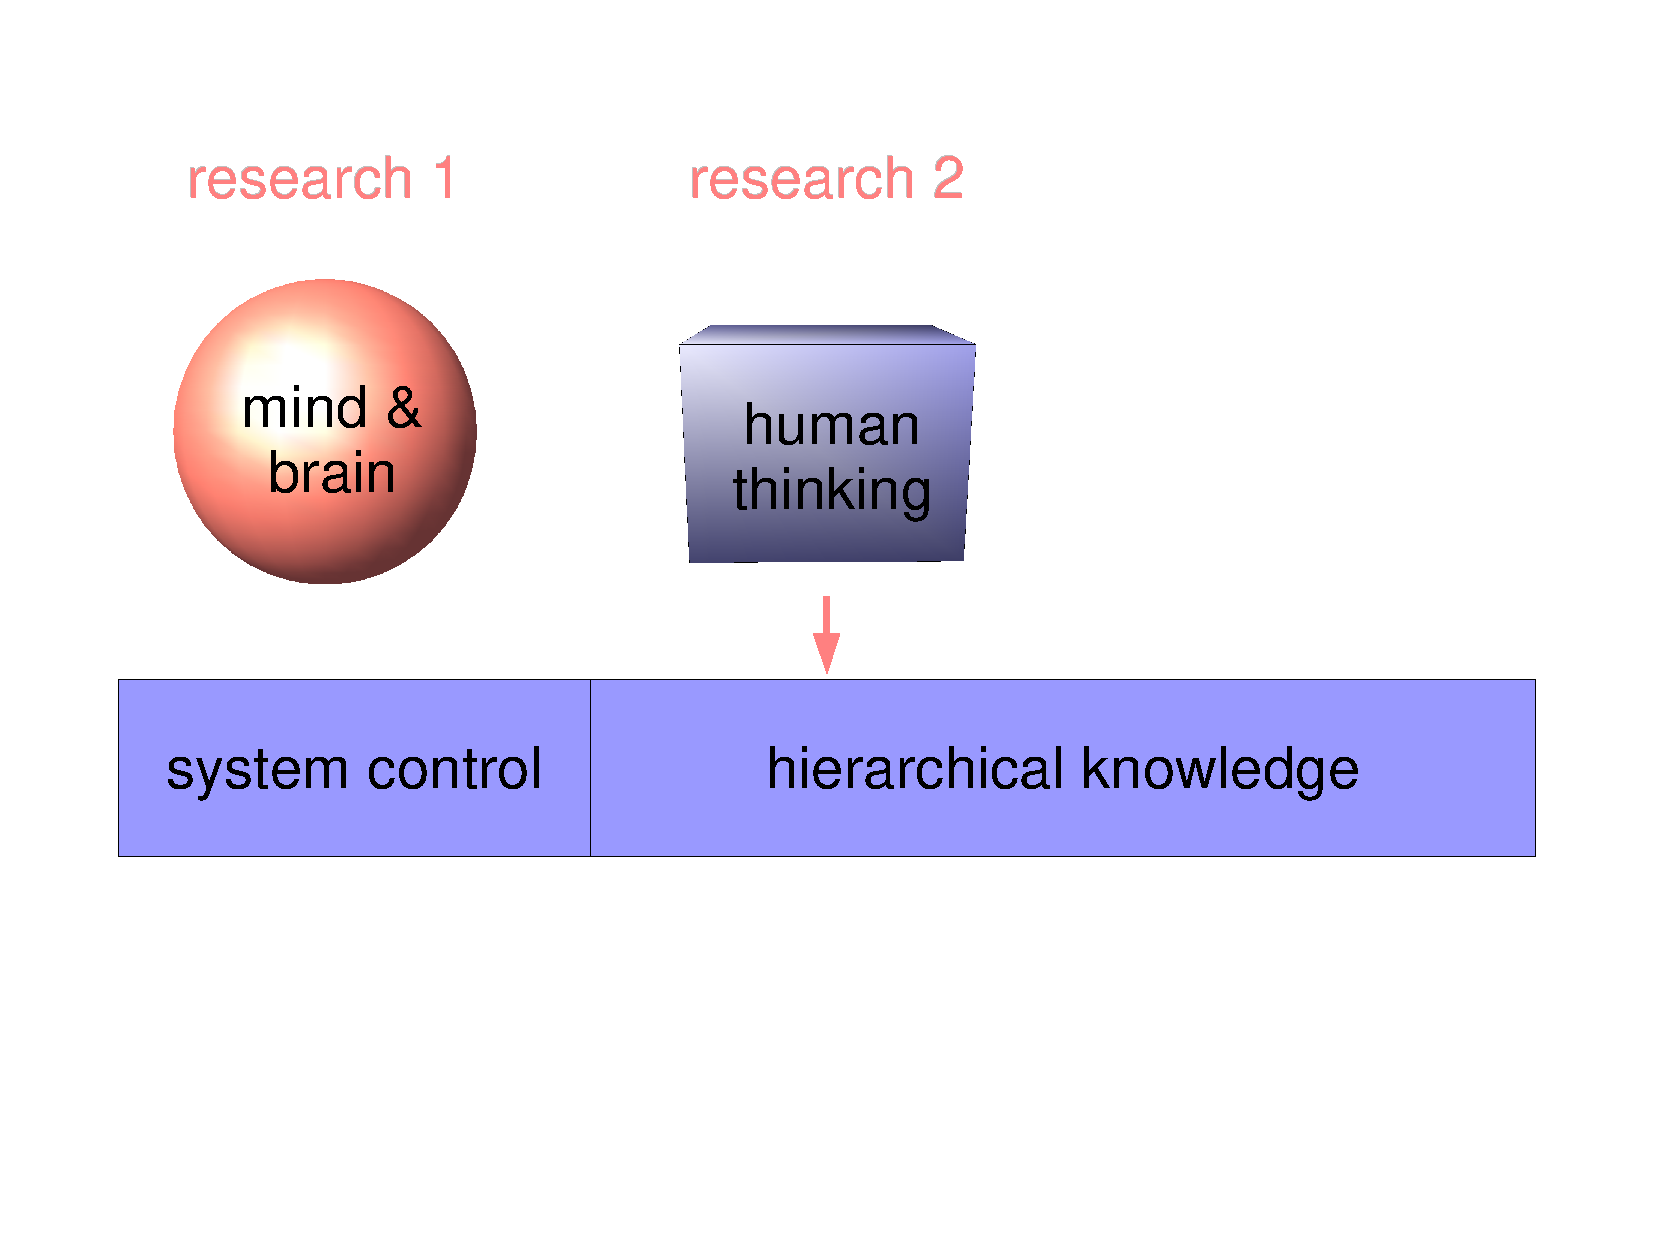
\includegraphics[scale=0.3,angle=-90]{graphic/hierarchicalknowledge.pdf}
        \caption{Concepts of Human Thinking Leading to Hierarchical Knowledge}
        \label{hierarchicalknowledge_figure}
    \end{center}
\end{figure}

Through the application of these thoughts, the knowledge becomes
\emph{Hierarchical Knowledge} (figure \ref{hierarchicalknowledge_figure}).
Additionally, this work tries to embed knowledge models in an environment of
\emph{Dimensions}, as known from physics, and further properties. Every model
keeps a number of \emph{Meta Information} about its parts. \emph{Positions} in
space or time are one such example.

Chapter \ref{knowledge_schema_heading} further elaborates on these issues.
